\documentclass{standalone}
\usepackage{tikz}
\usetikzlibrary{patterns}
%\usetikzlibrary{...}
\begin{document}
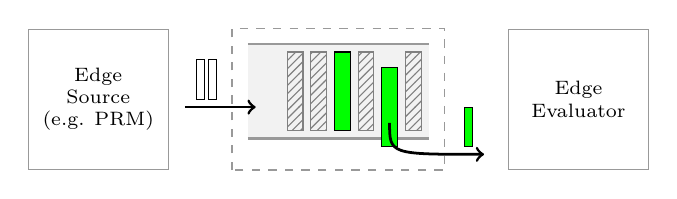
\begin{tikzpicture}
\node[rectangle,draw=black!40,minimum size=0.7in] at (-2.2, -0.1) {
   \parbox{1.5cm}{\scriptsize\centering Edge\\Source\\(e.g. PRM)}};
\draw[fill=black!5,draw=none] (-0.3,-0.6) rectangle (2.0,0.6);
\draw[line width=1pt,color=black!40] (-0.3,-0.6) -- (2.0,-0.6);
\draw[line width=1pt,color=black!40] (-0.3, 0.6) -- (2.0, 0.6);
\draw[line width=0.5pt,color=black!40,dashed] (-0.5,-1.0) rectangle (2.2,0.8);
\draw[pattern=north east lines, pattern color=black!50, draw=black!50] (0.2,-0.5) rectangle (0.4,0.5);
\draw[pattern=north east lines, pattern color=black!50, draw=black!50] (0.5,-0.5) rectangle (0.7,0.5);
\draw[fill=green] (0.8,-0.5) rectangle (1.0,0.5);
\draw[pattern=north east lines, pattern color=black!50, draw=black!50] (1.1,-0.5) rectangle (1.3,0.5);
\draw[fill=green] (1.4,-0.7) rectangle (1.6,0.3);
\draw[pattern=north east lines, pattern color=black!50, draw=black!50] (1.7,-0.5) rectangle (1.9,0.5);
\draw[line width=1pt,->] (-1.1,-0.2) -- (-0.2,-0.2);
\draw[] (-0.95,-0.1) rectangle (-0.85,0.4);
\draw[] (-0.8,-0.1) rectangle (-0.7,0.4);
\draw[line width=1pt,->] (1.5, -0.4) .. controls(1.5, -0.8) .. (2.7, -0.8);
\draw[fill=green] (2.45,-0.7) rectangle (2.55,-0.2);
\node[rectangle,draw=black!40,minimum size=0.7in] at (3.9, -0.1) {
   \parbox{1.5cm}{\scriptsize\centering Edge\\Evaluator}};
\end{tikzpicture}
\end{document}
